Now with our effective potential in hand we look for an extrema of the potential:
\begin{align*}
	r_\text{ext} &= \frac{l^2}{2M}\left[1\pm\sqrt{1 - 12\left(\frac{M}{l}\right)^2}\right]
\end{align*}
We now consider what happens to this in some strange conditions. If we set $\frac{l}{M} < \sqrt{12}$, then we see this will have imaginary solutions (which implies the extrema vanish).
Only the larger solution will be stable, so we are more interested in this solution.

\subsection{Radial plunge}
We consider radial freefall from $r=\infty$ starting at rest. Therefore $l = 0$, $u^t = 1$, from our killing vector we know:
\begin{align*}
	e &= \left(1 - \frac{2M}{r}\right)u^t \\
	1 &= \left(1 - \frac{2M}{r}\right)u^t 
\end{align*}
We also know:
\begin{align*}
	\frac{e^2-1}{2} &= \frac{1}{2} u^r\ ^2 - \frac{M}{r} \\
	-\sqrt{\frac{2M}{r}} &= r \\
	\sqrt{r} dr &= -\sqrt{2M} d\tau \\
	u &= \left[ \left(1- \frac{2M}{r}\right)^{-1}, -\sqrt{\frac{2M}{r}}, 0, 0\right] \\
	- \frac{2}{3}r^\frac{3}{2} &= -\sqrt{2M}(\tau_* - \tau) & r(\tau_*) &= 0 \\
	r(\tau) &= \left(\frac{3}{2}\right)^\frac{2}{3} (2M)^\frac{1}{3}(\tau_* - \tau)^\frac{2}{3}
\end{align*}
We now look to find our coordinate time $t$:
\begin{align*}
	e &= \left(1 - \frac{2M}{r}\right)u^t \\
	\frac{dt}{d\tau} &= \left(1 - \frac{2M}{r}\right)^{-1} \\
	\frac{dt}{dr} &= -\left(1 - \frac{2M}{r}\right)^{-1}\left(\frac{2M}{r}\right)^{-\frac{1}{2}} \\
	t &= t_* + 2M\left[ -\frac{2}{3}\left(\frac{r}{2M}\right)^\frac{3}{2} - 2\left(\frac{r}{2M}\right)^\frac{1}{2} + \log|\frac{\sqrt{\frac{r}{2M}} + 1}{\sqrt{\frac{r}{2M}} - 1} |\right]
\end{align*}

\subsection{Stable circular orbits}
We can say that our stable circular orbit ocur with $r=r_\text{ext}$ which decreases with decreasing $\frac{l}{m}$, and we see that the minimum it has is $r_\text{SCO} = 6M$.
We can see that the angular velocities ($\Omega$) in circular orbits (defined relative to a distant observer):
\begin{align*}
	\Omega &= \frac{d\phi}{dt} \\
	\Omega &= \frac{u^\phi}{u^t} \\
	\Omega &= \frac{1}{r^2} \left(1 - 2\frac{M}{r}\right) \frac{l}{e}
\end{align*}
This gives us a relation between $r$ and $l$ using our potential at the minimum, and additionally we see:
\begin{align*}
	e^2 &= \left(1-\frac{2M}{r}\right)\left(1 + \frac{l^2}{r^2}\right) \\
	r_\text{min} &= \frac{l^2}{2M} \left[ 1 + \sqrt{1 - 12\frac{M^2}{l^2}}\right] \\
	\varepsilon &= \frac{1}{2} u^r\ ^2 + V_\text{eff}
\end{align*}
So:
\begin{align*}
	\frac{l}{e} &= \sqrt{Mr} \left(1 - \frac{2M}{r}\right)^{-1} \\
	\Omega^2 &= \frac{M}{r^3}
\end{align*}
Which is Kepler's law!

We now want to look at null trajectories in the Schrwarzchild geometry. We will parameterize this curve using an affine parameter $\lambda$, with the for velocity normalized to $u_\alpha u^\alpha = 0$.
We have the same killing vectors so:
\begin{align*}
	e &= \left( 1 \frac{2M}{r}\right) \frac{dt}{d\lambda} \\
	l &= r^2\sin^2\theta\frac{d\phi}{d\lambda}
\end{align*}
W.L.O.G. we consider the equitorial plane $\theta = \frac{\pi}{2}$:
\begin{align*}
	-\left(1 - \frac{2M}{r}\right)u^t\ ^2 + \left(1 -\frac{2M}{r}\right)^{-1} u^r\ ^2 + r^2u^\phi\ ^2 &=0 \\
	-\left(1 - \frac{2M}{r}\right)^{-1}e^2 + \left(1 -\frac{2M}{r}\right)^{-1} u^r\ ^2 + \frac{l^2}{r^2} &=0 \\
	\frac{1}{b^2} &= \frac{1}{l^2} u^r\ ^2 + W_\text{eff} \\
	b^2 &= \frac{l^2}{e^2} & W_\text{eff} &= \frac{1}{r^2} \left(1- \frac{2M}{r}\right)
\end{align*}
If we consider a light ray moving parallel to the x axis at some displacement above the x-axis $d$:
\begin{figure*}[h]
	\centering
	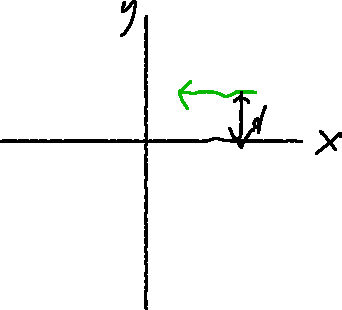
\includegraphics[width=6cm]{2-04-1.png}
	\caption*{The trajectory of light in our example}
\end{figure*}
\begin{align*}
	x &= r\cos\phi & y &= r\sin\phi \\
	b &= r^2 u^\phi
\end{align*}
And we say approximately:
\begin{align*}
	\phi &\approx \frac{d}{r} & \frac{dr}{dt} &= -1 & \frac{d\phi}{dt} &= \frac{d}{r^2}
\end{align*}
